%\documentclass{article}
\documentclass{scrartcl}
\usepackage[utf8]{inputenc}
\usepackage[bottom]{footmisc}
\usepackage{amsmath,amsthm,amssymb}
\usepackage{algorithmic}
\usepackage{algorithm}
\usepackage{xcolor}
\usepackage{rotating}
\usepackage{listings}
\usepackage{enumitem}
\usepackage{graphicx}
\usepackage[colorlinks = true,
            linkcolor = black,
            urlcolor  = blue,
            citecolor = black,
            anchorcolor = blue]{hyperref}
\setlength\parindent{0pt}

\def\imp{\rightarrow}

\newenvironment{level}%
{\addtolength{\itemindent}{2em}}%
{\addtolength{\itemindent}{-2em}}


\newtheorem{theorem}{Theorem}[section]
\newtheorem{corollary}{Corollary}[theorem]
\newtheorem{lemma}[theorem]{Lemma}



\makeatletter
\newcommand{\inlineitem}[1][]{%
\ifnum\enit@type=\tw@
    {\descriptionlabel{#1}}
  \hspace{\labelsep}%
\else
  \ifnum\enit@type=\z@
       \refstepcounter{\@listctr}\fi
    \quad\@itemlabel\hspace{\labelsep}%
\fi}
\makeatother

\definecolor{mGreen}{rgb}{0,0.6,0}
\definecolor{mGray}{rgb}{0.5,0.5,0.5}
\definecolor{backgroundColour}{rgb}{0.95,0.95,0.92}

\lstset{
    backgroundcolor=\color{backgroundColour},   
    commentstyle=\color{mGreen},
    keywordstyle=\color{blue},
    numberstyle=\tiny\color{mGray},
    stringstyle=\color{gray},
    basicstyle=\footnotesize,
    breakatwhitespace=false,         
    breaklines=true,                 
    captionpos=b,                    
    keepspaces=true,                 
    numbers=left,                    
    numbersep=5pt,                  
    showspaces=false,                
    showstringspaces=false,
    showtabs=false,                  
    tabsize=2,
    language=C
}


\title{POP SS19 Homework 2 Documentation}
\subtitle{Robert Ernstbrunner, 01403753}

\begin{document}
\maketitle

\textit{Since I cannot attend the next lecture to present my work I tried my best to explain in great detail what was done here.}

\section*{Introduction}

In this assignment the abstract syntax tree (\textit{AST}) for executable statements of \textit{C} functions had to be build. To verify the correctness of the \textit{AST} the output was visualized with help of the \textit{dot} language and the \textit{graphviz} environment. This document describes the structure of the \textit{AST} and gives a general overview of the implementation.

\section*{AST structure}
The structure of the abstract syntax tree as well as the interface for generating the \textit{AST} and \textit{dot} file are defined in the \texttt{intermediate.h} header file (Figure~\ref{lst:header}).\\

\subsection*{struct ast}
The struct of the tree can be observed in lines 4 - 10 in Figure~\ref{lst:header}. The naming conventions are similar to those in the \textit{Flex and Bison} guide \cite{bison}.\\
I decided to build a binary (instead of a ternary) tree. Each node comprises a \textit{nodetype} of type \texttt{\textcolor{blue}{int}} that indicates whether the node is a decision node (\textit{nodetype} = '$D$' for decision node)\footnote{Notice the implicit type conversion from \texttt{\textcolor{blue}{char}} to \texttt{\textcolor{blue}{int}}.}, a leaf node of type \texttt{\textcolor{blue}{double}} (\textit{nodetype} = '$C$' for constant) or a leaf node of type \texttt{\textcolor{blue}{char *}} (\textit{nodetype} = '$I$' for identifier).\\
Decision nodes store their label in the \texttt{\textcolor{blue}{char *}} variable and either the left or right or both pointers to subtrees are set. Leaf nodes either assign the \texttt{\textcolor{blue}{char *}} or the \texttt{\textcolor{blue}{double}} variable and the pointers to subtrees are set to \texttt{\textcolor{blue}{NULL}}.\\

\subsection*{interface description}
\begin{itemize}

\item The \textit{newast(\ldots)} method creates and returns a decision node. Thus, it needs a label and a left and right subtree as input (where one of them can be set to \texttt{\textcolor{blue}{NULL}}).

\item The \textit{newnum(\ldots)} method creates and returns a leaf with a \texttt{\textcolor{blue}{double}} value. This method is called whenever a \texttt{CONSTANT} is returned from the lexer.

\item The \textit{newid(\ldots)} method creates and returns a leaf with a \texttt{\textcolor{blue}{char *}} value. This method is called whenever it is appropriate, e.g., when an \texttt{IDENTIFIER} or keyword is returned from the lexer.

\item The \textit{generate\_dot(\ldots)} method creates the \texttt{test\_function.dot} file. It then makes one call to \textit{write\_tree(\ldots)} and thereby starts a chain of recursive calls that fill up the \texttt{test\_function.dot} file with nodes and edges.

\item The \textit{write\_tree(\ldots)} method labels nodes and the \textit{write\_node(\ldots)} method links nodes. Both routines call each other recursively until every node has been visited in a depth first search manner.\\
As long as the current node is not a leaf node the \textit{write\_tree(\ldots)} method computes either the number of the left child node with \texttt{2 $\cdot$ nodenum}\footnote{\texttt{nodenum} denotes the current node number and is 1 for the root node.} or the number of the right child node with \texttt{2 $\cdot$ nodenum + 1}, or, in case of two subtrees, both and then calls the \textit{write\_node(\ldots)} routine(s) accordingly. After linking the parent node to the current node the \textit{write\_node(\ldots)} method calls the \textit{write\_tree(\ldots)} method again. This approach was inspired by the bison calculator by Jim Mahoney\cite{calc}.

\item The \textit{free\_tree(\ldots)} method frees all the nodes that were allocated during the parsing process. Unfortunately, a check with \textit{Valgrind} indicates that some memory is directly lost and I couldn't fix this issue in time.

\end{itemize}

\begin{figure}[H]
\lstinputlisting{intermediate.h}
\caption{itermediate header file}
\label{lst:header}
\end{figure}

\section*{Design decisions}

\subsection*{Parser.y}
The parser.y file is probably the most interesting file in this assignment. It contains three sections (declarations, rules and auxiliary procedures) and is the central component for parsing.
\paragraph*{declarations}
In order to be able to return a complete parse tree of type \textit{struct ast*} in the main function of the third section, an additional parameter for the \textit{yyparse(\ldots)} method in line 9 of Figure~\ref{lst:declarations} has to be defined. This also affects the definition of \textit{yyerror(\ldots)} in line 6 where the same parameter must be incorporated. The debug variable in line 8 is later used in the auxiliary procedures section and will therefore be explained later on.\\
The \textit{\%union} construct in lines 13 - 17 is used to tell bison what symbols have what types of values.\footnote{the default value is \texttt{\textcolor{blue}{int}}.} E.g., the \texttt{CONSTANT} token in line 19 is assigned the value \textit{d} of type \texttt{\textcolor{blue}{double}} with the $<$ $>$ command. The types (nonterminals) \textit{primary\_expression} and \textit{additive\_expression} get the value \textit{astree} of type \textit{struct ast*} in line 22. 

\paragraph*{rules}  In the rules section probably most of the 'dull' work was done. Out of the countless rules I highlight just one typical example in Figure~\ref{lst:rules}. Right besides the derivation in line 4 the dollar-notation in brackets is used to link the nonterminal \textit{statement} (represented by \$1) of type \textit{struct ast*} to the rest of the tree (represented by \$\$). On the further right I defined some debug output for when the debug flag in section three is set. In order to link multiple statements in the \textit{AST} the \textit{newast(\ldots)} method is used to create a new \texttt{STATEMENT} node labeled \texttt{'STMT'}.\\
The root of the \textit{AST} was set by defining an additional entry point. In lines 8-9 the \textit{external\_declaration} symbol derives to the \textit{parse\_tree} symbol and the \textit{AST} is set in the brackets to the right. \texttt{parse\_tree} is then derived to the same symbols as the \texttt{eternal\_declaration} usually would. This (supposedly) does not affect the functionality of the grammar. However, it should be mentioned that the entry point might be set a bit too high in the parse hierarchy and could be moved further down.

\paragraph*{auxiliary procedures} In this section the main method is defined. First of all, a parameter for custom debug output was added in lines 10 - 12 in Figure~\ref{lst:auxprod}. Furthermore, the \textit{AST} struct is declared in line 14 and its address is given to \textit{yyparse}. After successful parsing the \textit{AST} is passed on to the \textit{generate\_dot(\ldots)} method in order to produce the \textit{test\_function.dot} file. Afterwards all the allocated memory is (supposedly) freed with the \textit{free\_tree(\ldots)} method.

\begin{figure}[H]
\begin{lstlisting}[escapeinside={(*}{*)}]
// declarations
(*\ldots*)
%{
#include "intermediate.h"
(*\ldots*)
int yyerror(struct ast **astree, char *s);

int debug = 0;
%}

%parse-param {struct ast **astree}

%union {
  struct ast *astree;
  double d;
	char *id;
}

%token <d> CONSTANT (*\ldots*)
%token <id> IDENTIFIER STRING_LITERAL SIZEOF (*\ldots*)
(*\ldots*)
%type <astree> primary_expression additive_expression (*\ldots*)
(*\ldots*)
%% // rules
\end{lstlisting}
\caption{declarations (parser.y)}
\label{lst:declarations}
\end{figure}

\begin{figure}[H]
\begin{lstlisting}[escapeinside={(*}{*)}]
%% // rules
	(*\ldots*)
statement_list
	: statement	{ $$ = $1; if(debug)printf("statement_list : statement\n"); }
	| statement_list statement { $$ = newast("STMT", $1, $2); }
	;
	(*\ldots*)
external_declaration
	: parse_tree { *astree = $1; }
	;
	
parse_tree
	: function_definition
	| declaration
	;
	(*\ldots*)		
%% // auxiliary procedures
\end{lstlisting}
\caption{rules (parser.y)}
\label{lst:rules}
\end{figure}

\begin{figure}[H]
\begin{lstlisting}[escapeinside={(*}{*)}]
%% // auxiliary procedures
(*\ldots*)
int main(int argc, char **argv)
{
	(*\ldots*)
			 /********************************/
       /* specify your own option here */
       /********************************/					
				
				case 'd':
					debug = 1;
					break;
	(*\ldots*)	
	struct ast *astree;
	yyresult = yyparse(&astree);
	(*\ldots*)	
	generate_dot(astree);
	free_tree(astree);
	(*\ldots*)
}
\end{lstlisting}
\caption{auxiliary procedures (parser.y)}
\label{lst:auxprod}
\end{figure}

\section*{Function evaluation and visualization}

The non trivial test function that was used as example for the \textit{AST} is outlined in Figure~\ref{fig:func}. I incorporated \texttt{IF}, \texttt{IF ELSE}, \texttt{SWITCH}, \texttt{FOR}, \texttt{WHILE} and \texttt{DO WHILE} statements which can be compound and nested as well.\\

The \texttt{makefile} from the first assignment was used and extended with the rule\\

\texttt{\textcolor{red}{png}:}\\
\-\qquad \texttt{dot -Tpng  test\_function.dot -o test\_function.png}\\

in order to produce the \textit{.png} file from the \textit{.dot} file. Finally, the visualization of the \textit{AST} is presented in Figure~\ref{fig:ast}.
The abort condition of the \texttt{WHILE} and \texttt{FOR} statements is given in the left subtree while the compound statement of the \texttt{WHILE} and \texttt{FOR} statements is linked as the right subtree. For the \texttt{DO WHILE} statement the branches are switched so that the abort condition is represented in the right subtree. This is due to the fact that, in order to read the code in the right order, the \textit{AST} must be traversed in DFS from left to right. Also, while the subtree for the \texttt{IF} statement without \texttt{ELSE} branch is structurally similar to the \texttt{FOR}/ \texttt{WHILE} statements, the \texttt{IF ELSE} statement probably needs further explanation. The root of this statement is the \texttt{IF} node. To the left is the condition while to the right there is another node denoted as \texttt{<- IF | ELSE ->} that comprises the \texttt{IF} part in the left subtree and the \texttt{ELSE} part in the right subtree.

\section*{Additional notes}
The \textit{scanner} should also be mentioned, since it had to be adapted form the first assignment as well. Initially, the \textit{scanner} only returned tokens, but not the values that belonged to them. Therefore, in some cases, the \textit{yytext} value had to be stored in the specified values of \textit{yylval}, i.e., for \texttt{IDENTIFIERES} the content from \textit{yytext} was stored in \textit{yylval.id} and for \texttt{CONSTANTS} the value from \textit{yytext} was stored in \textit{yylval.d}.\\

\paragraph{The makefile} should be used by typing
\begin{enumerate}
\item \texttt{make} (to build the \textit{cparser} executable)
\item \texttt{./cparser test\_function.c} (to create the \textit{.dot} file)
\item \texttt{make png} (to create the \textit{.png} file)
\item \texttt{make clean\_all} (to clean everything)
\end{enumerate}
\begin{figure}[H]
\lstinputlisting{test_function.c}
\caption{evaluated function \textit{func}}
\label{fig:func}
\end{figure}

\begin{sidewaysfigure}
	\centering
	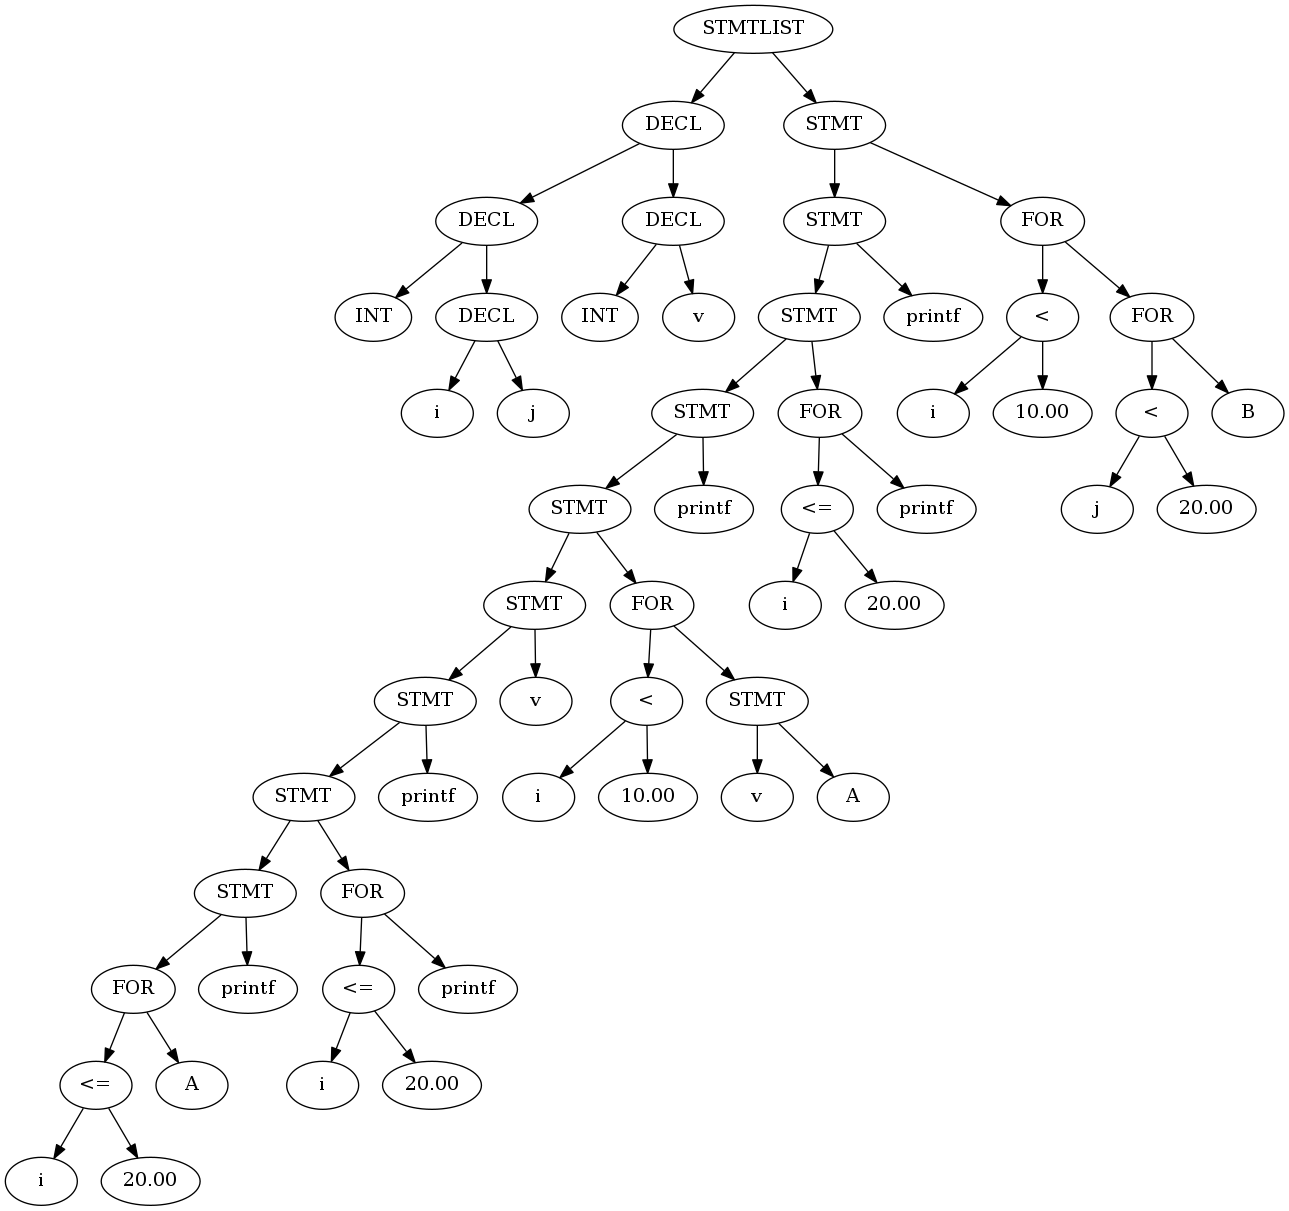
\includegraphics[width=\paperwidth]{test_function.eps}
	\caption{the \textit{AST} for the function \textit{func} in Figure~\ref{fig:func}.}
	\label{fig:ast}
\end{sidewaysfigure}

\bibliographystyle{plain}
\bibliography{Documentation}
\end{document}
